\documentclass[a4paper,12pt]{article}

\usepackage{geometry}
\geometry{
paper = a4paper,
%margin = 2cm,
%hmargin={2cm, 1cm},
left = 2cm,
right = 2cm,
top = 2cm,
bottom = 3cm
}

\usepackage{xcolor}
\usepackage{graphicx}

\usepackage{amsmath}

\usepackage{hyperref}

\hypersetup{
colorlinks = true,
linkcolor = blue
}

\begin{document}
	
\title{\textbf{How to get started with \LaTeX?}}
\author{Dr. David Raj Micheal}
\date{02 June, 2020}

\maketitle

\begin{abstract}
Lorem ipsum dolor sit amet, consectetur adipiscing elit. Vestibulum pellentesque vel quam sit amet scelerisque. Integer in nunc ante. Ut mattis sem ac ligula bibendum, non laoreet tellus pharetra. Sed rhoncus lacus eu velit dictum blandit. Duis venenatis lorem in tincidunt ullamcorper. Proin sagittis faucibus fringilla. Nunc porttitor urna nibh, vel vestibulum magna cursus vitae. Ut luctus nibh metus, vel feugiat ipsum iaculis nec. Fusce congue, mauris sed aliquam efficitur, turpis massa pharetra mauris, id imperdiet eros nunc vel nunc. Ut fringilla, lectus ac eleifend condimentum, dui urna mollis lorem, eget tincidunt lacus ipsum sollicitudin nibh. Vestibulum at turpis quis sapien pulvinar pretium. Quisque sit amet tristique erat, eget auctor urna. Pellentesque at nisl id augue placerat scelerisque eget quis quam. Aliquam eget eleifend magna, eget facilisis lacus. Proin eget scelerisque ante, ac ultricies nulla.
\end{abstract}

\tableofcontents


\section{Introduction}

Praesent et ex sed orci egestas molestie eu non ante. Pellentesque id pulvinar nibh. Etiam sed lectus tortor. Vivamus et elit quis velit sollicitudin hendrerit vitae nec ligula. In sed pellentesque ipsum, eget maximus tellus. Sed efficitur cursus nisl sed cursus. Sed eleifend nisi at est mattis molestie. Integer id diam vehicula lectus blandit dapibus nec scelerisque ipsum. Nunc vestibulum dui non dictum fermentum. Nulla volutpat justo mi, ac volutpat risus malesuada eget. Donec semper eu sem vitae eleifend. Lorem ipsum dolor sit amet, consectetur adipiscing elit. Proin et erat ac odio semper commodo. Vestibulum ligula nibh, vestibulum ac felis et, blandit venenatis sem. Class aptent taciti sociosqu ad litora torquent per conubia nostra, per inceptos himenaeos. \cite{arthur2003}.


\section{How to insert math equations?}

	The formula to find roots of a given quadratic equaiton is given by, $\frac{-b\pm\sqrt{b^2-4ac}}{2a}$. You can give it in display mode as well \cite{querty_1996}.
	
\subsection{Equation environment}
	Ut ut neque et dolor cursus scelerisque. Suspendisse aliquam mi in justo vulputate, non luctus ipsum lacinia. Proin at lacinia neque. Cras sem erat, malesuada rutrum condimentum vel, suscipit et lacus. Sed ultricies id odio et molestie. Maecenas vestibulum lacinia metus, quis commodo nunc varius at. Nulla pulvinar faucibus tellus nec ullamcorper. Donec convallis tellus vitae velit commodo vestibulum.
		\begin{equation}
			\frac{-b\pm\sqrt{b^2-4ac}}{2a}
		\end{equation}
		
\subsection{Align environment}
Lorem ipsum dolor sit amet, consectetur adipiscing elit. Nunc sem turpis, gravida non erat sed, semper placerat mauris. Praesent pulvinar, nulla et egestas porttitor, nulla tellus faucibus purus, tincidunt tincidunt augue eros dictum nisi. Vestibulum fringilla dignissim urna id molestie. Nulla facilisi. Suspendisse et tempor augue. Ut ut tortor ac nulla pulvinar dictum. Praesent mollis fringilla suscipit. Nullam mattis ullamcorper vulputate.
\begin{align}
	f(x) & = x^2 -5x + 6 \\
		 & = (x-3)(x-2)
\end{align}

Nunc elementum felis quis libero lacinia tristique. Sed in dapibus velit, nec ultrices metus. Suspendisse potenti. Curabitur vitae felis facilisis, malesuada neque tempor, sollicitudin elit. Donec egestas dignissim nisl eu ullamcorper. Integer imperdiet, ante nec varius pretium, dolor turpis dictum velit, eget blandit augue sem sit amet odio. Proin mollis turpis lorem. Maecenas id sapien in eros maximus volutpat at ut libero. Cras auctor dui ipsum, ac facilisis nulla blandit vitae. Vivamus dictum rhoncus odio ut lobortis.

\section{How to insert images?}


\begin{figure}[htb!]
	\centering
	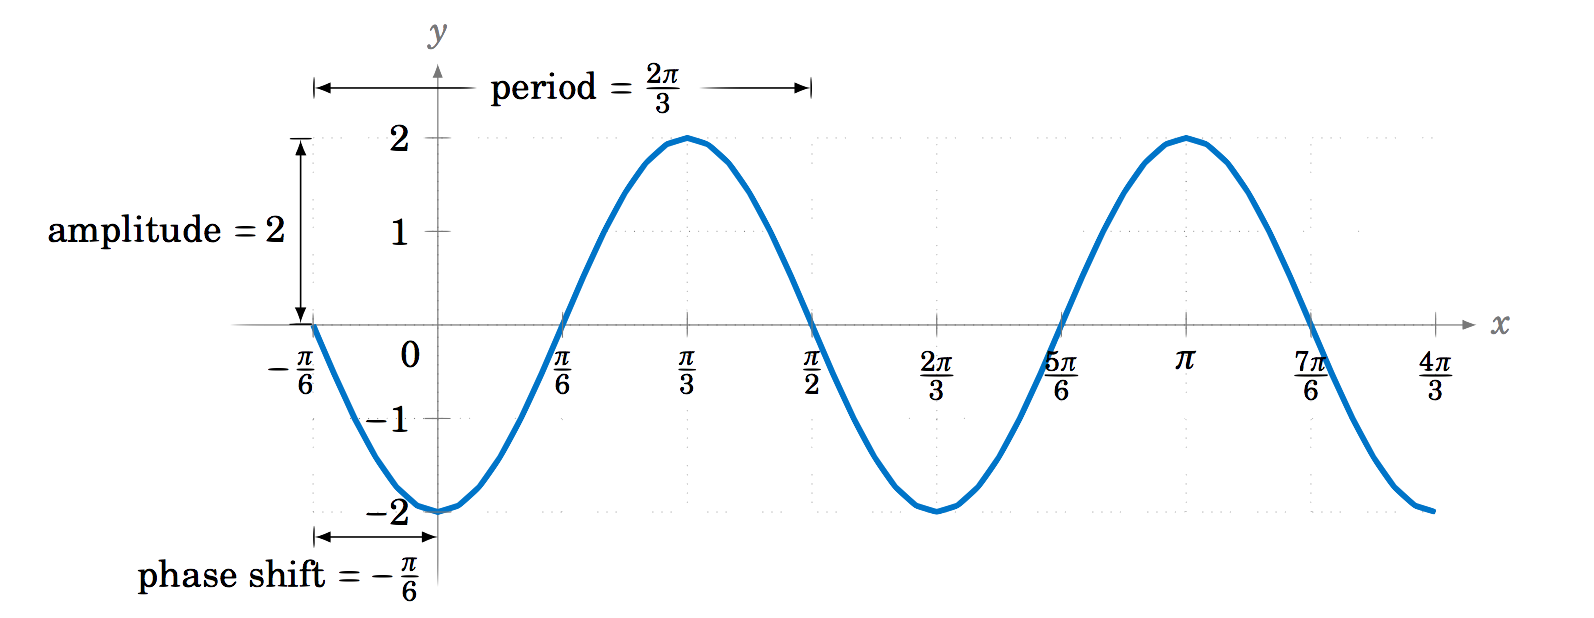
\includegraphics[scale=.5]{img/sin-graph}
	\caption{Graph of $\sin x$}
	\label{fig:sinx}
\end{figure}
Here we will see how to insert images by inserting the \autoref{fig:sinx}. 
Nam ac turpis at sapien tempus gravida ac in dolor. Vestibulum ante ipsum primis in faucibus orci luctus et ultrices posuere cubilia curae; Phasellus pretium at ligula dignissim gravida. Nullam turpis enim, suscipit eu tempor non, varius eget lorem. Aliquam mollis leo at aliquam auctor. Mauris vel mauris lectus. Etiam facilisis orci id tellus hendrerit malesuada ac ut quam. Nunc convallis congue venenatis. Phasellus magna risus, rutrum a facilisis et, sagittis eget ligula. Duis sagittis odio fermentum arcu tincidunt, nec consectetur odio bibendum. Fusce at condimentum leo, non rutrum nibh. Vivamus vestibulum augue vitae sem euismod interdum. Duis elementum dui sed lobortis semper. \cite{napster_1998}


\section{How to create table in \LaTeX}

Vivamus nec mauris et ipsum lacinia maximus. Phasellus eu arcu sed magna tristique elementum id et neque. Nullam dapibus sed lectus nec eleifend. Phasellus pretium nisl in nibh auctor, non porttitor eros pretium. Suspendisse blandit hendrerit facilisis. Quisque tristique non ex lobortis auctor. Phasellus consectetur scelerisque ultricies. Mauris ac lacinia velit, ac tristique mi. Vestibulum pellentesque, diam feugiat tristique interdum, nibh arcu bibendum tortor, sit amet maximus neque ex ut quam. Phasellus pretium in sapien vel lacinia. In quis tortor at dui lobortis posuere eget in ante. Proin quis dui at mi sollicitudin interdum sed eget leo. Ut euismod nunc sapien, eget accumsan nibh cursus sit amet. Maecenas maximus congue diam in bibendum.

\begin{table}[htb!]
	\renewcommand{\arraystretch}{1.25}
	\centering
	\begin{tabular}{|l|l|}
		\hline
		\textbf{Name}   & \textbf{Email}                     \\ \hline
		Keiko C. Young  &  young@gmail.com    \\
		Ainsley J. Roth & roth@gmail.com \\
		Armand M. Webb  &  webb@gmail.com\\
		Jana G. Mercer  &  mercer@gmail.com     \\ \hline
	\end{tabular}
\caption{Names and Emails of my customers}
\label{tab:customers}
\end{table}

In the \autoref{tab:customers}, we have listed our customers.





\bibliographystyle{plain}
\bibliography{references}

\end{document}